\section{Historia}

El termino \emph{gamification} fue acuñado cerca del año 2008\cite{DefineGamefication}. 
El objetivo fue crear un termino que concentrara todas las ideas y o elementos utilizados en el 
diseño de juegos que se pudiesen traspasar a otros contextos, distintos a los de entretencion. 
En el año 2010 este termino llega a ser tan utilizado que aparecio como \emph{trend} en google\cite{LiCap1.3}.

El concepto basico fue inicialmente utilizado en la decada de los ochenta con el objetivo 
de mejorar y actualizar el juego llamado \emph{MUD}, \emph{Multy User Dungeons}. El desarrollador, 
Richard Bartle, comenzo a analizar a los jugadores en donde encontro 4 estereotipos \ref{fig:Players}.

Con esta informacion, modifico el juego para satisfacer cada tipo de jugador encontrado. Esto tuvo un 
gran exito y demostro una nueva forma de enganchar a los clientes, esto llamo la atencion de  
empresas que vieron este concepto como una nueva forma de atraer y retener a sus clientes.

\begin{figure}[!htb]
  \centering
  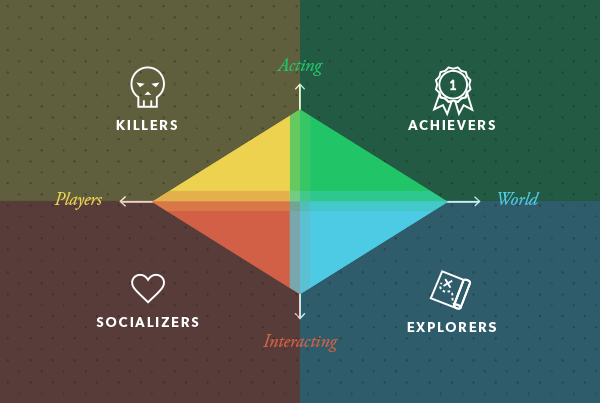
\includegraphics[width=0.5\textwidth]{images/TypeOfPlayersBartle.png}
  \caption[Caption for LOF]{Real caption\footnotemark}
  \label{fig:Players}
\end{figure}

\footnotetext{Source: \url{http://www.example.com/theimage.png}}


Diversas compañias actualmente usan esta tecnica, varias de estas han creado plataformas para aplicar gamification.
En $2007$, la compañia \emph{Bunchball} \footnote{www.bunchball.com} fue una de las primeras en implementar y proveer
una plataforma gamificada como un servicio\cite{Gam:Bunchball:1}. \emph{Bunchball} tuvo clientes de gran tamaño como
Bravo\footnote{www.bravotv.com} y \emph{The USA network}\footnote{www.usanetwork.com}\cite{Gam:Bunchball:2}.

Otras grandes empresas que utilizan gamificaion en la actualidad son: SAP AG, IBM, EMC, CA, Slalom Consulting,
 Deloitte, Microsoft, LiveOps, RedCritter\cite{Gam:Companies:1}  

Actualmente se han creado eventos acerca de esta tecnica como \emph{Gamification 2013}, un evento de discucion sobre
el futuro de gamification\cite{Gam:Events:1}. En $2014$ se llevara a cabo \emph{Loyalty Gamification World Championship} en San Franscico, USA.\cite{Gam:Events:2}

\section{Definicion}

Hoy en dia \emph{gamification} se ha convertido en una herramienta para las empresas 
para poder captar mas clientes. Cada dia aumenta el uso de este concepto por lo que es
necesario entregar una definicion apropiada para el concepto.  \emph{Gamification} se puede definir
como el uso de elementos del diseño de juego en contextos diferentes al de juego. Para entender mejor 
los conceptos bajo esta definicion se explicara por partes:

\begin{itemize}

\item Juego: En primer lugar este concepto se refiere al juego, en su todo, y no a la accion de jugar.
Este concepto es caracterizado por un conjunto de reglas explicitas que crean un ambiente  
en donde los jugadores buscan la competicion para completar objetivos y metas.

\item Elementos del diseño de juego: Dentro de este concepto se puede encontrar 2 definiciones.
La primera, es una definicion estricta que solo acepta ciertos elementos unicos. La segunda, 
es una definicion en donde todos los elementos pueden ser utilizados. Para llegar a una 
definicion robusta es necesario juntar ambas y asi obtener un conjunto mas restrictivo en donde 
los elementos a utilizar son carateristicos a los juegos, que se encuentran en la mayoria de estos y 
que cumplen una rol importante en la jugabilidad de estos.

\item Contextos diferentes al de juego: Este es el concepto mas complejo de explicar debido a que es una idea  
abstracta. Una forma de explicarla es como una situacion de la vida cotidiana que existe fuera 
de un juego o de un ambiente que contiene \emph{gamification}.

\end{itemize}

\section{Utilizacion}

Gamification has been widely applied in marketing. Over 70 of Forbes Global 2000 companies surveyed in 2013 said they planned to use gamification for the purposes of marketing and customer retention.[24] For example, in November 2011 Australian broadcast and online media partnership Yahoo!7 launched its Fango mobile app, which TV viewers use to interact with shows via techniques like check-ins and badges. As of February 2012, the app had been downloaded more than 200,000 times since its launch.[25] Gamification has also been used in customer loyalty programmes. In 2010, Starbucks gave custom Foursquare badges to people who checked in at multiple locations and offered discounts to people who became mayors of an individual store.[26] There have also been proposals to use gamification for competitive intelligence,[27] encouraging people to fill out surveys,[28] and to do market research on brand recognition.[29] Gamification has also been integrated into Help Desk software. In 2012, Freshdesk, a SaaS-based customer support product, integrated gamification features, allowing agents to earn badges based on performance.[30]

Gamification has also been used as a tool for customer engagement,[31] and for encouraging desirable website usage behavior.[19] Additionally, gamification is readily applicable to increasing engagement on sites built on social network services. For example, in August 2010, one site, DevHub, announced that they have increased the number of users who completed their online tasks from 10 to 80 after adding gamification elements.[32] On the programming question-and-answer site Stack Overflow users receive points and/or badges for performing a variety of actions, including spreading links to questions and answers via Facebook and Twitter. A large number of different badges are available, and when a user's reputation points exceed various thresholds, he or she gains additional privileges, including at the higher end, the privilege of helping to moderate the site.

Gamification can be used for ideation, the structured brainstorming to produce new ideas. A study at MIT Sloan found that ideation games helped participants generate more and better ideas, and compared it to gauging the influence of academic papers by the numbers of citations received in subsequent research.[33]

Education and training are areas where there has been interest in gamification.[35][36] Microsoft released the game Ribbon Hero 2 as an add-on to their Office productivity suite to help train people to use it effectively,[37] which was described by Microsoft as one of the most popular projects its Office Labs division ever released.[38] The New York City Department of Education with funding from the MacArthur Foundation and the Bill and Melinda Gates Foundation has set up a school called Quest to Learn centred around game-based learning, with the intent to make education more engaging and relevant to modern kids.[39] SAP has used games to educate their employees on sustainability.[40] The US military and Unilever have also used gamification in their training.[41] The Khan Academy is an example of the use of gamification techniques in online education.[42] In August 2009, Gbanga launched the educational location-based game Gbanga Zooh for Zurich Zoo that asked participants to actively save endangered animals and physically bring them back to a zoo. Players maintained virtual habitats across the Canton of Zurich to attract and collect endangered species of animals.[43] In 2014, the True Life Game project was initiated, with the main purpose of researching the best ways to apply concepts of gamification and crowdsourcing into lifelong learning.

Applications like Fitocracy and QUENTIQ use gamification to encourage their users to exercise more effectively and improve their overall health. Users are awarded varying numbers of points for activities they perform in their workouts and gain levels based on points collected. Users can also complete quests (sets of related activities) and gain achievement badges for fitness milestones.[44] Health Month adds aspects of social gaming by allowing successful users to restore points to users who have failed to meet certain goals.

Employee productivity is another problem that gamification has been used to tackle. RedCritter Tracker,[45] Playcall,[46] and Arcaris [47] are examples of management tools that use gamification to improve productivity. Digital Brand Group is the first company in India to fully gamify their work process to make their work style more engaging and encouraging.

Crowdsourcing has been gamified in games like Foldit, a game designed by the University of Washington, in which players compete to manipulate proteins into more efficient structures. A 2010 paper in science journal Nature credited Foldit's 57,000 players with providing useful results that matched or outperformed algorithmically computed solutions.[48] The ESP Game is a game that is used to generate image metadata. Google Image Labeler is a version of the ESP Game that Google has licensed to generate its own image metadata.[49] Research from the University of Bonn used gamification to increase wiki contributions by 62.[50]

Experts anticipate that the technique would also be applied to health care, financial services, transportation, government,[51] employee training,[41] and other activities.[52]

Alix Levine, an American security consultant, described gamification as some techniques that a number of extremist websites such as Stormfront and various terrorism-related sites used to build loyalty and participation. As an example, Levine mentioned reputation scores.[53][54] The Anti-Defamation League has noted that some terror groups, such as Hezbollah, have created actual games to market their ideology to adolescents.[55]

Microsoft has also announced plans to use gamification techniques for its Windows Phone 7 operating system design.[56]

Gamification has also been applied to authentication. For example, the possibilities of using a game like Guitar Hero can help someone learn a password implicitly.[57] Furthermore, games have been explored as a way to learn new and complicated passwords. It is suggested that these games could be used to "level up" a password, thereby improving its strength over time.[58] Gamification has also been proposed as a way to select and manage archives.[59] Recently, an Australian technology company called Wynbox has recorded success in the application of its gamification engine to the hotel booking process.[60]




